\chapter{Results}
This chapter discusses the results of our project. A description of the built application will be given, alongside with screenshots.
Also, graphs will be used to show the performance of our application.

\section{SwiftTV}
Since we built a download and stream application for the Samsung SmartTV based on libswift, we dubbed our application SwiftTV.
The name is kept simple because other existing applications based on libswift have similar names. This section explains how SwiftTV works.

\begin{center}
\begin{figure}[h!]
	\centering
	\mbox{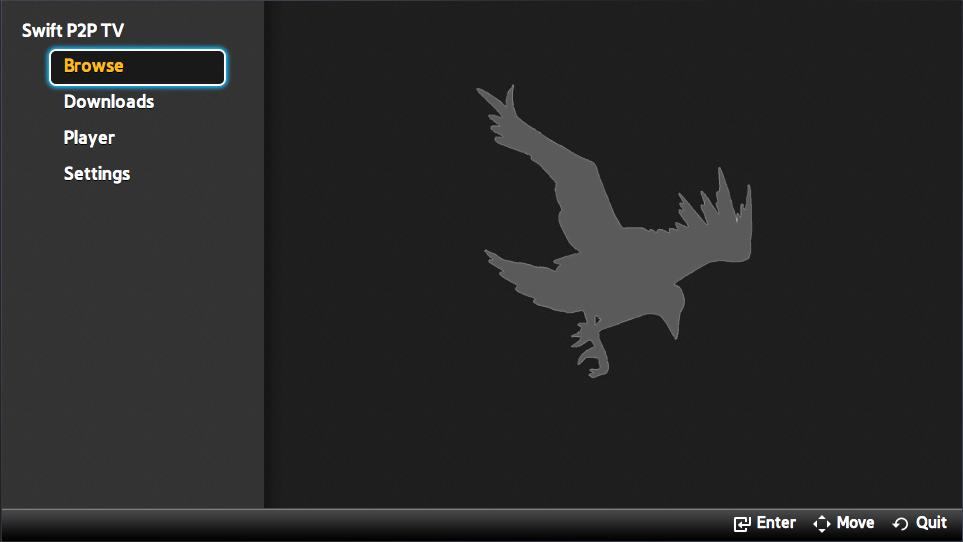
\includegraphics[width=0.8\textwidth]{Images/MainScene.jpg}}
	\label{fig:main}
	\caption{Screenshot of the Main scene.}
\end{figure}
\end{center}

The \hyperref[fig:main]{main menu} points to the four different pages in the application, browse, downloads, player and settings. When selecting one of these pages the main menu remains visible.

\begin{center}
\begin{figure}[h]
	\centering
	\mbox{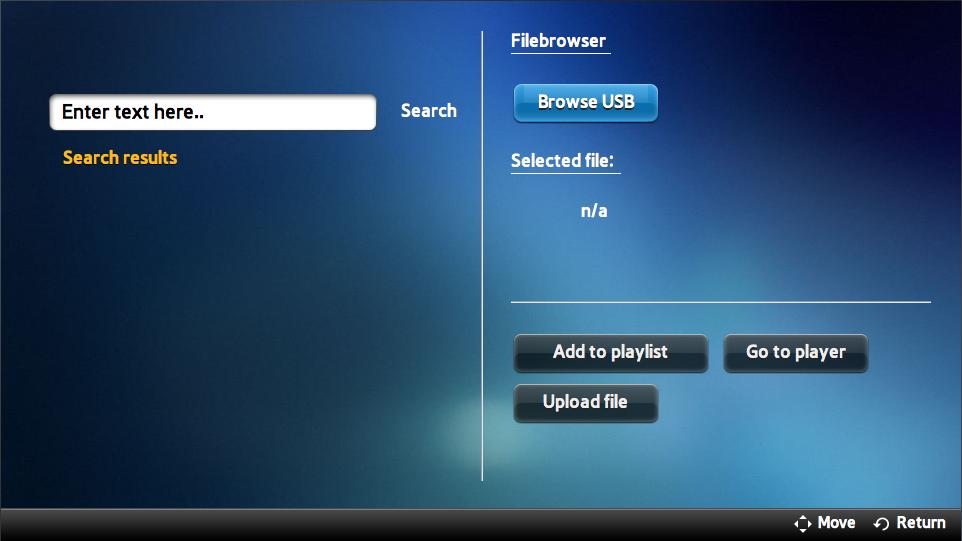
\includegraphics[width=0.8\textwidth]{Images/BrowseScene.jpg}}
	\label{fig:browse}
	\caption{Screenshot of the Browse scene.}
\end{figure}
\end{center}

\hyperref[fig:browse]{Browse} is where you can either browse your local filesystem to play a media file or search the internet for files to download or stream. Browsing the local filesystem is done with features included in the Samsung API and is therefor all done in JavaScript. When choosing a file from the browser it can be added to the playlist in the player page to be played. The search functionality sends a "/search:searchTerm" request to the HTTP server which in turn starts a search using Dispersy. After some time the search results are requested by JavaScript using a ``/results'' request. The results are returned in the form of an XML file and shown on screen. 

The user can select one of these results and choose to either download ot stream it. JavaScript either sends a ``/add:hash'' or ``/stream:hash request'' depending on the choice. If download is chosen the the download is added to the list in DownloadManager and start downloading. If stream is chosen a stream is opened and is added to the playlist on the player page.

\begin{center}
\begin{figure}[h]
	\centering
	\mbox{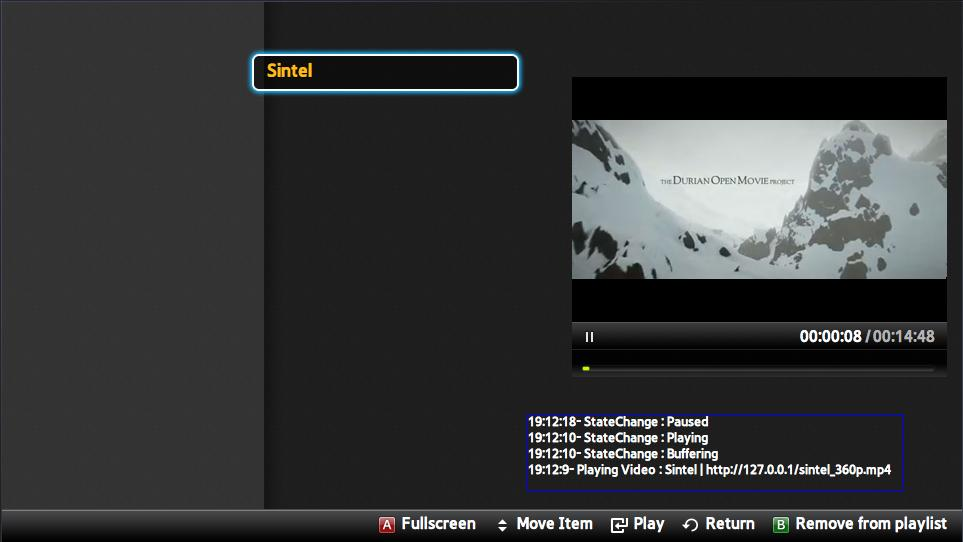
\includegraphics[width=0.8\textwidth]{Images/PlayerScene.jpg}}
	\label{fig:player}
	\caption{Screenshot of the Media Player scene.}
\end{figure}
\end{center}

\hyperref[fig:player]{Player} is where videos and streams can be viewed. To view videos or streams they must first be added to the playlist while in the browser. Videos will start playing in the small screen but full screen can be enabled afterwards.

\begin{center}
\begin{figure}[h]
	\centering
	\mbox{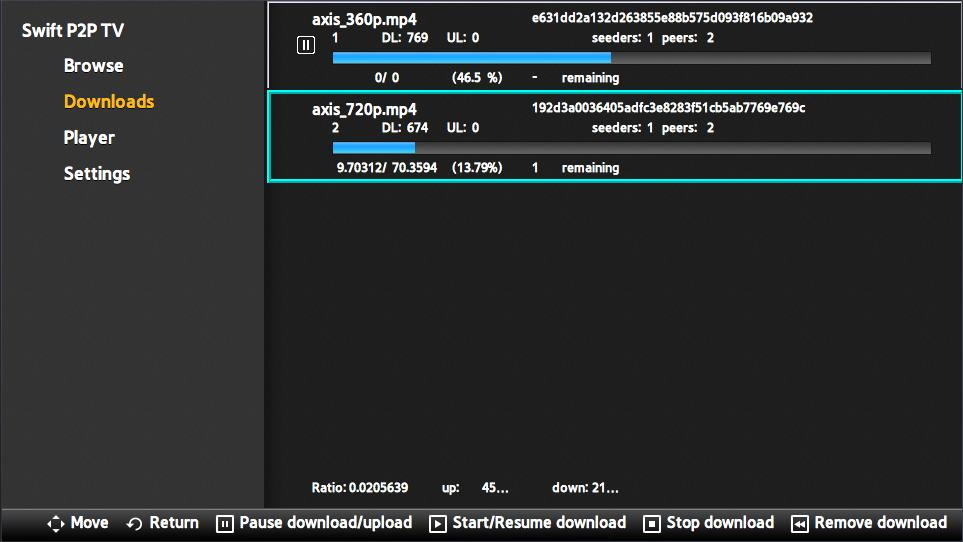
\includegraphics[width=0.8\textwidth]{Images/DownloadsScene.jpg}}
	\label{fig:downloads}
	\caption{Screenshot of the Downloads scene.}
\end{figure}
\end{center}

\hyperref[fig:downloads]{Downloads} is where the current list of downloads can be viewed. Downloads can be paused, stopped and resumed. JavasScript will send ``/pause:hash'', ``/remove:hash'' and ``/resume:hash'' requests to do this.
When stopping a download it will be removed from the list.

\begin{center}
\begin{figure}[h]
	\centering
	\mbox{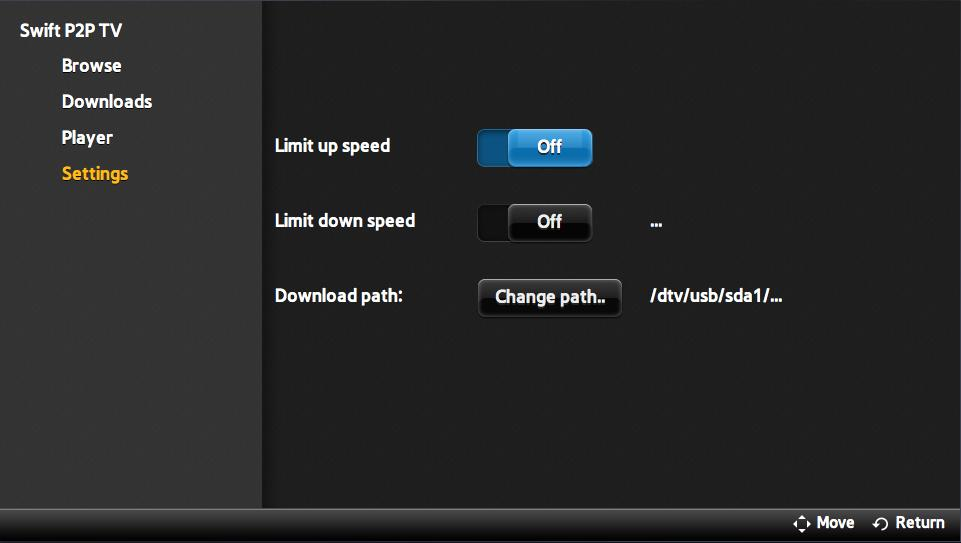
\includegraphics[width=0.8\textwidth]{Images/SettingsScene.jpg}}
	\label{fig:settings}
	\caption{Screenshot of the Settings scene.}
\end{figure}
\end{center}

In the \hyperref[fig:settings]{settings page} users can set their maximum download and upload speed as well as the download location. These settings are saved in memory and loaded on startup. When the settings are changed JavaScript sends a ``/settings:upspeed:downspeed:downloadpath'' request to the HTTP server.

\section{Measurements}
For this section, we measured the CPU and memory usage of the application against the time.
This way, we can see how much resources our application needs. The measurements were done on a Samsung D7000
TV, \footnote{\url{http://www.samsung.com/uk/consumer/tv-audio-video/television/led-tv/UE40D7000LUXXU}} while playing a stream.
The Sintel video\ref{fig:sintel} was used for the tests. Several measurements were made, where we varied the download speed limits for the streams.
Then the same measurements were done for the total CPU and memory usage, so we can see how much resources the TV needs in total while running
our application. Also, measurements were taken while the TV was being idle, to show the exact differences between normal circumstances and situations
that require more CPU and memory resources.
\clearpage
\begin{center}
\begin{figure}[h!]
	\centering
	\mbox{
\includegraphics[width=0.6\textwidth]{Images/sintel.jpg}}
	\caption{Screenshot of the video used. Video and screenshot are made by the developers of the Sintel project.}
	\label{fig:sintel}
\end{figure}
\end{center}

\scalebox{0.6}{
\lstinputlisting{Images/mediainfo.txt}
}
\clearpage

\subsection{Memory/CPU usage of SwiftTV}

\begin{center}
\begin{figure}[h]
	\centering
	\mbox{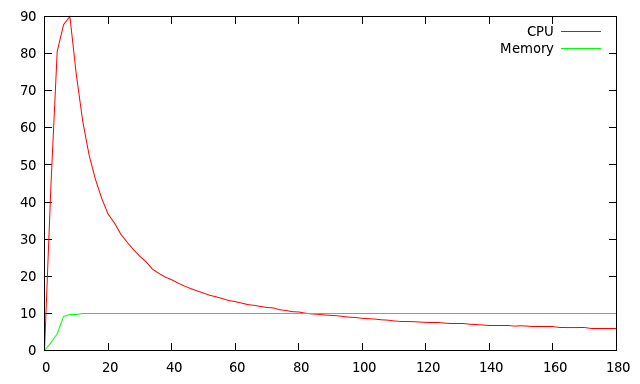
\includegraphics[width=1.2\textwidth]{Images/idle.png}}
	\caption{CPU and memory usage of the application, while being idle.}
	\label{graph:idle}
\end{figure}
\end{center}

\begin{center}
\begin{figure}[h]
	\centering
	\mbox{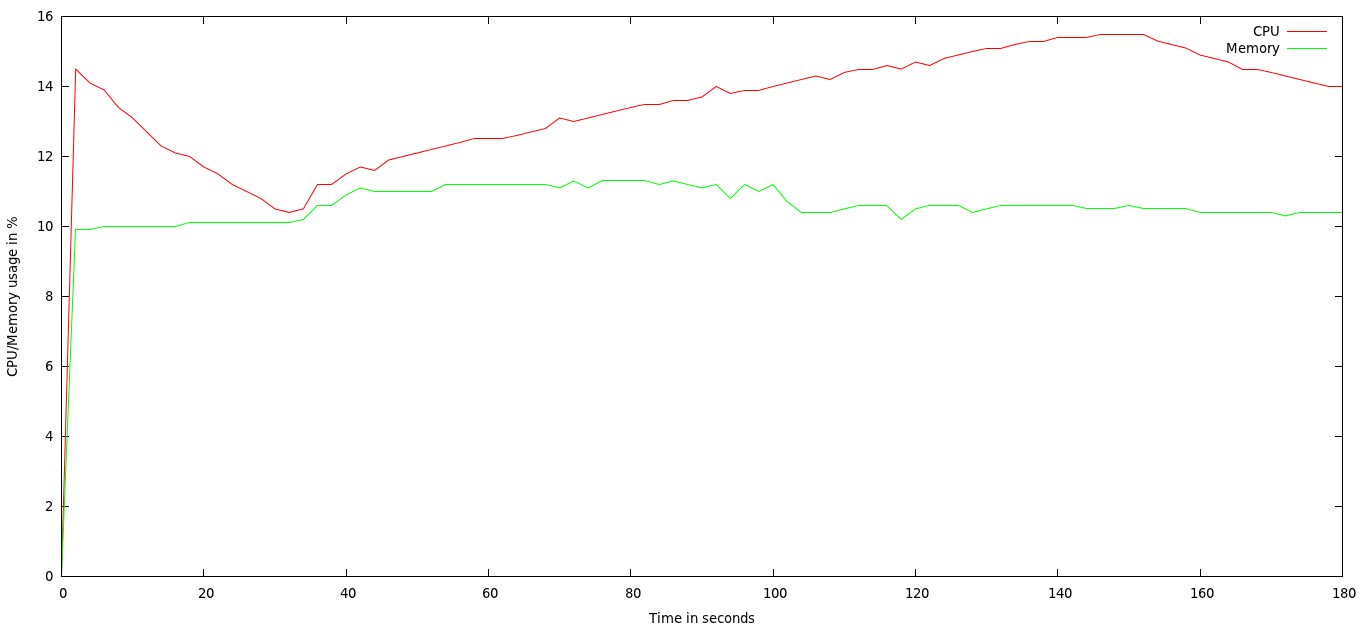
\includegraphics[width=1.2\textwidth]{Images/500kbs.png}}
	\caption{CPU and memory usage while streaming at 500 kB/s.}
	\label{graph:500kbs}
\end{figure}
\end{center}

\begin{center}
\begin{figure}[h]
	\centering
	\mbox{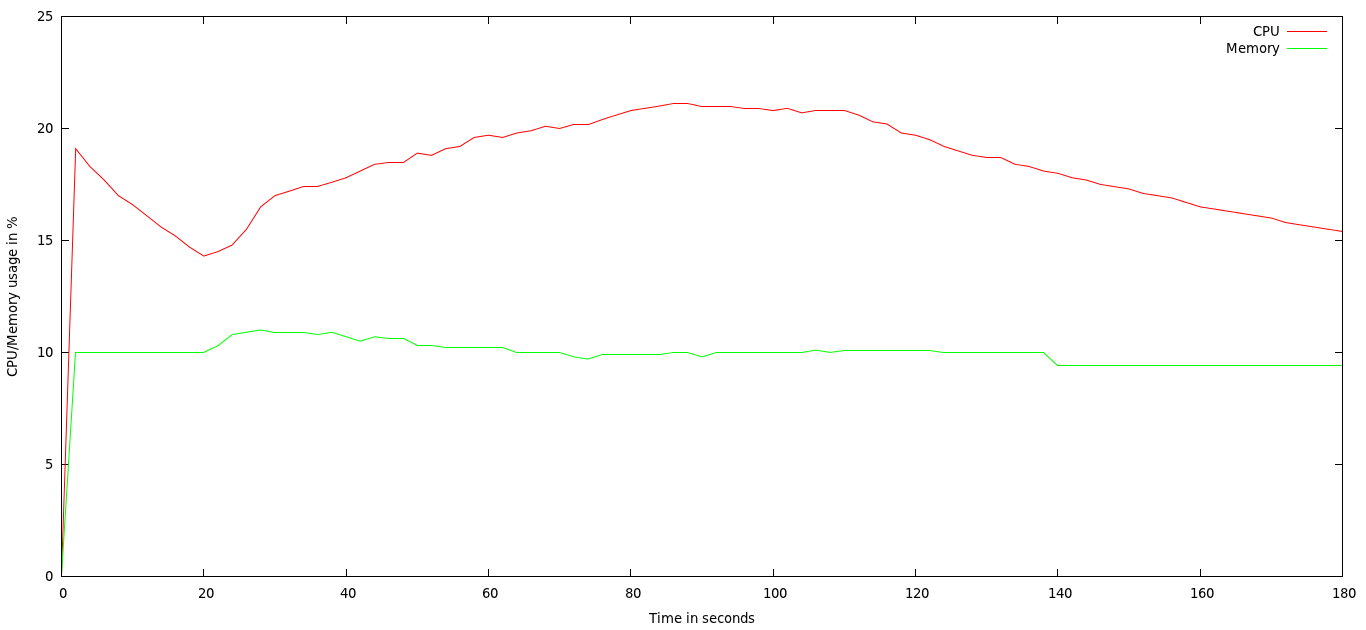
\includegraphics[width=1.2\textwidth]{Images/700kbs.png}}
	\caption{CPU and memory usage while streaming at 700 kB/s. This is also the bitrate of the video used. \ref{fig:sintel}}
	\label{graph:700kbs}
\end{figure}
\end{center}

\begin{center}
\begin{figure}[h]
	\centering
	\mbox{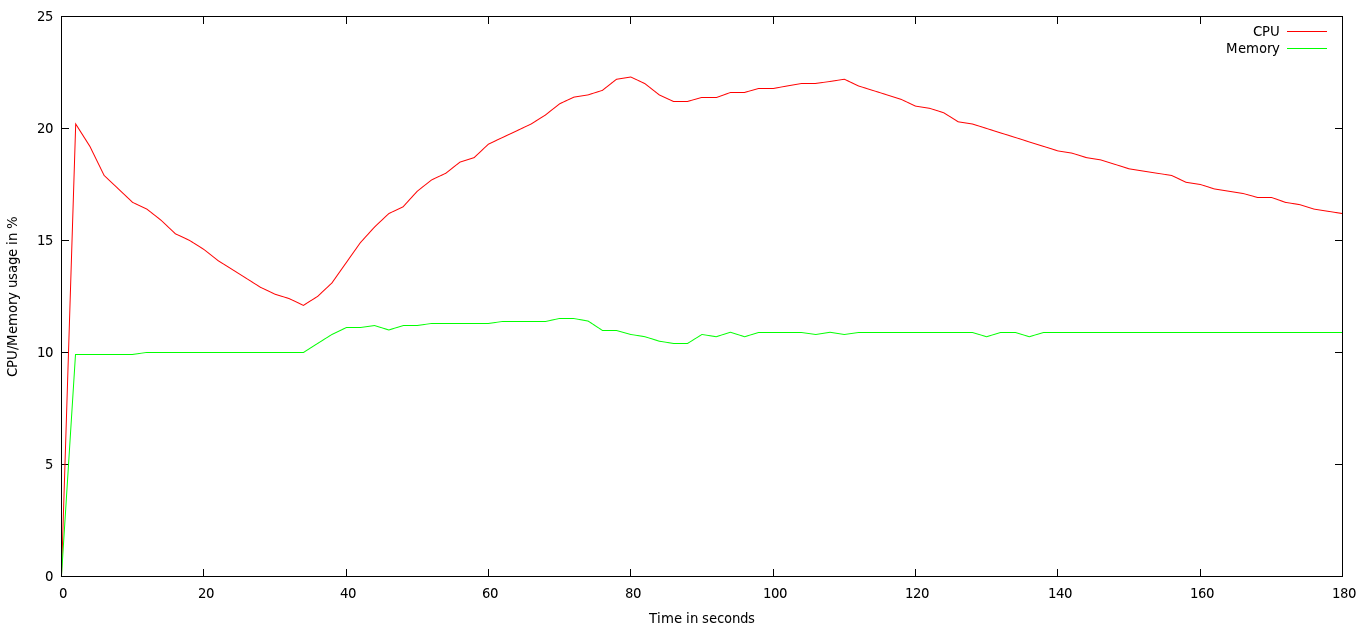
\includegraphics[width=1.2\textwidth]{Images/1000kbs.png}}
	\caption{CPU and memory usage while streaming at 1 MB/s.}
	\label{graph:1Mbs}
\end{figure}
\end{center}
\clearpage

Figure \ref{graph:idle} shows the CPU and memory usage of only the application, while being 
idle.
The peak in the beginning depicts the initialisation of the application, where modules such 
as Dispersy are started up.
Figure \ref{graph:500kbs} shows the CPU and memory usage while streaming the video at 500 
kB/s. It can be seen that the CPU usage is
always under 16\%, while this upper limit grows with the bitrate we set, as shown in 
\ref{graph:700kbs} and \ref{graph:1Mbs}.

As expected, the lower the bitrate, the lower the CPU usage. However, the memory usage 
always stays the same, even when the application is idle. This goes against our 
expectations of memory usage of getting progressively higher the faster you stream. This 
means that our goal of limiting the memory usage to 256 MB has been achieved, since the TV 
has 350 MB of RAM, while we are only using 10\% of it. Our goal of having a response time 
of 300 ms has not been achieved, however. From our own experience, we see that the 
application responds too slow (between 1 and 2 seconds). Even though we allowed the 
program to use 100\% of CPU resources, we see that this was not even necessary since it 
only uses up to 23\% when streaming at 1 MB/s.

\subsection{Total CPU/Memory usage}
TODO: The same graphs, but then for the total CPU/Memory usage of the TV while running the application.